\chapter{Sensitivity and noise}
\label{ch:sensitivity}

\section{The readout-window optimum}
\label{sec:window}

From 92 ODMR sweeps at 17 readout windows on 2026-08-06
(\file{docs/2026-08-06\_twopoint\_timing/tables/integration\_time.csv}). Lorentzian
fits over 2840--2900\,MHz; noise taken from the point-to-point scatter of the
off-resonance wings, which is immune to slow drift across the sweep.

\begin{center}
\small
\begin{tabular}{@{}rrrrrrr@{}}
\toprule
\hd{$\tau$ (\us)} & \hd{contrast} & \hd{$\sigma_z$} & \hd{$\sigma_z\sqrt{\tau}$} & \hd{$\sigma(\Delta f)$ kHz} & \hd{$t_\text{rep}$ \us} & \hd{$\eta$ \etaunit} \\
\midrule
50  & 0.541 & 3.01e-3 & 0.0213 & 51.3 & 109 & $186\pm14$ \\
90  & 0.517 & 2.13e-3 & 0.0202 & 37.0 & 189 & $\mathbf{177\pm14}$ \\
110 & 0.515 & 1.90e-3 & 0.0199 & 33.7 & 229 & $\mathbf{178\pm8}$ \\
\textbf{120} & 0.514 & 1.98e-3 & 0.0217 & 34.9 & 249 & $192\pm17$ \\
130 & 0.507 & 1.70e-3 & 0.0194 & 30.6 & 269 & $\mathbf{175\pm15}$ \\
140 & 0.506 & 1.71e-3 & 0.0202 & 30.6 & 289 & $181\pm7$ \\
170 & 0.513 & 2.01e-3 & 0.0262 & 35.6 & 349 & $232\pm5$ \\
190 & 0.495 & 2.09e-3 & 0.0288 & 38.4 & 389 & $264\pm22$ \\
\textbf{213} & 0.531 & 1.52e-3 & 0.0222 & 25.9 & 435 & $188\pm14$ \\
\bottomrule
\end{tabular}
\end{center}

Three results:

\begin{enumerate}
  \item \textbf{Contrast is flat} (0.49--0.54) across the whole range. A longer
        window buys no signal.
  \item \textbf{$\sigma_z\sqrt{\tau}$ is flat below $\sim$\SI{140}{\micro\second}
        (0.0207) and rises above it (0.0252).} Below \SI{140}{\micro\second} the
        readout averages down as $\sqrt{\text{time}}$; above it, the extra window
        length collects drift instead of statistics. \emph{This is the physical
        reason an optimum exists.}
  \item \textbf{$\eta$ is flat at $185\pm7$\,\etaunit\ for
        $\tau\le\SI{140}{\micro\second}$}, degrading to $232\pm20$ over
        150--\SI{200}{\micro\second}. Individual windows inside the flat band are
        not distinguishable --- the sweep-to-sweep scatter at fixed $\tau$ is
        $\pm14$, larger than the spread between them.
\end{enumerate}

\begin{figure}[H]
\centering
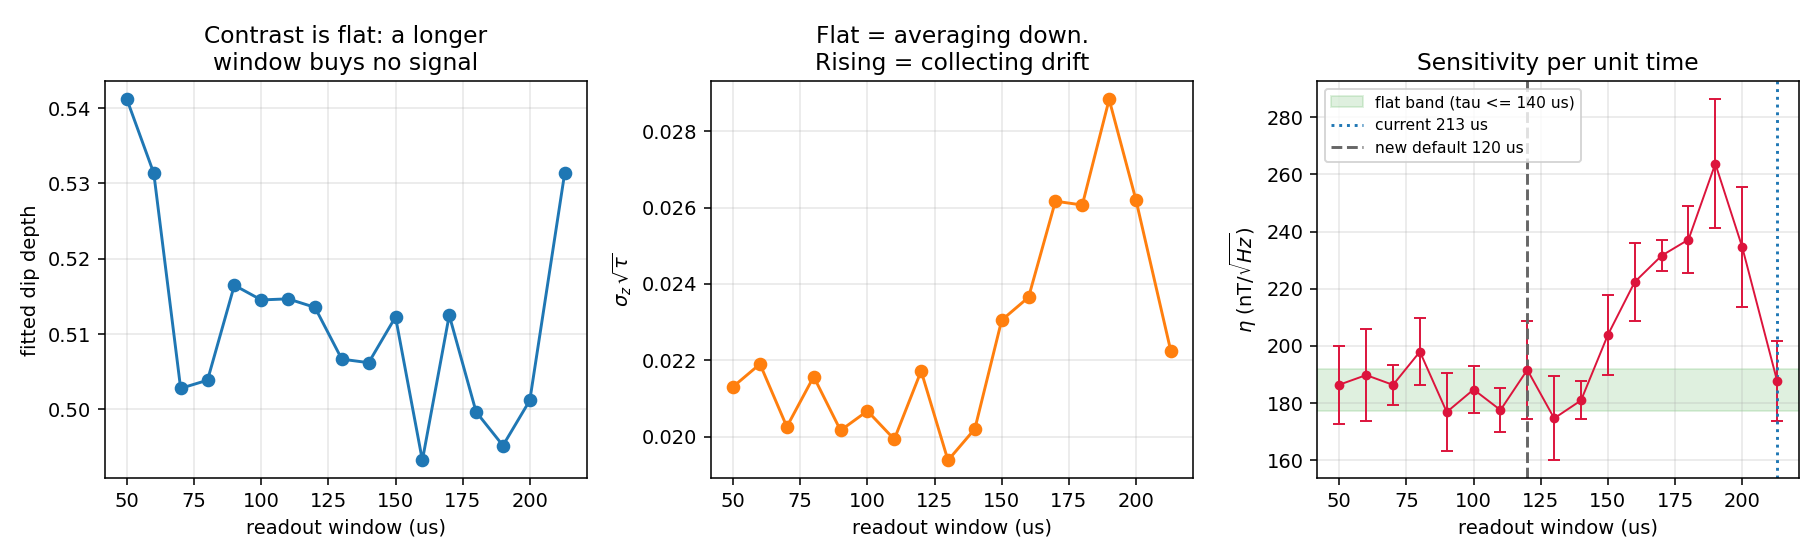
\includegraphics[width=\linewidth]{figures/integration_time.png}
\caption{Contrast, noise scaling and sensitivity against readout window, 2026-08-06.}
\end{figure}

\paragraph{Decision: $\tau = \SI{120}{\micro\second}$.} Inside the flat band, and
1.75$\times$ faster \emph{per rep} than \SI{213}{\micro\second}. Note carefully
that this does \textbf{not} make Method A faster (Chapter~\ref{ch:timing}) --- it
makes burst and streaming faster, and it lets more reps fit under Method A's call
floor.

\begin{openbox}[Two caveats that remain]
\textbf{The \SI{213}{\micro\second} point is an outlier.} It reads
188\,\etaunit, well below the 150--\SI{200}{\micro\second} trend it should
continue, on an unusually low $\sigma_z$ (1.52e-3). It was the configured default,
so those sweeps were probably taken under different conditions. The
$\sigma_z\sqrt{\tau}$ trend across 150--\SI{200}{\micro\second} is the more
reliable signal.

\textbf{The shape assumes \co{reps} was constant across the scan.} That is the
natural reading of a one-variable scan, and it is what flat $\sigma_z\sqrt{\tau}$
implies, but \co{reps} is not recorded in the sweep CSVs and cannot be recovered
from file timestamps (those gaps are dominated by operator cadence: median 4\,s
while $t_\text{rep}$ varies 4$\times$). A reps change part-way through could mimic
the rise above \SI{140}{\micro\second}.
\end{openbox}

\section{Measured sensitivity, per method}
\label{sec:etameas}

From \file{tables/modes.csv}. Both conventions of \S\ref{sec:conventions} are
given; when they disagree, trust the floor.

\begin{center}
\small
\begin{tabular}{@{}llrrrrr@{}}
\toprule
\hd{Session} & \hd{Method} & \hd{Run} & \hd{Rate} & \hd{$\sigma(\Delta f)$} & \hd{$\eta$} & \hd{Floor} \\
\midrule
08-14 & averaged & 144602 & 87.8\,Hz & 56.4\,kHz & 304 & 278 \\
08-14 & averaged & 144655 & 88.8\,Hz & 98.1\,kHz & 526 & 501 \\
08-14 & averaged & 145010 & 87.9\,Hz & 92.1\,kHz & 496 & 486 \\
08-14 & averaged & 145321 & 86.8\,Hz & 54.6\,kHz & 296 & 274 \\
08-14 & \textbf{stream} & 145442 & \textbf{1041.7\,Hz} & 160.8\,kHz & 251 & 240 \\
08-14 & \textbf{burst} & 150458 & 4166.7\,Hz (3089 net) & 71.4\,kHz & 56 & \textbf{38} \\
\midrule
08-06 & averaged & 144936 & 86.7\,Hz & 95.0\,kHz & 515 & 499 \\
08-06 & burst & 145051 & 2347\,Hz (2108 net) & 256.1\,kHz & 267 & 158 \\
\bottomrule
\end{tabular}
\end{center}
\emph{($\eta$ and floor in \etaunit.)}

\begin{figure}[H]
\centering
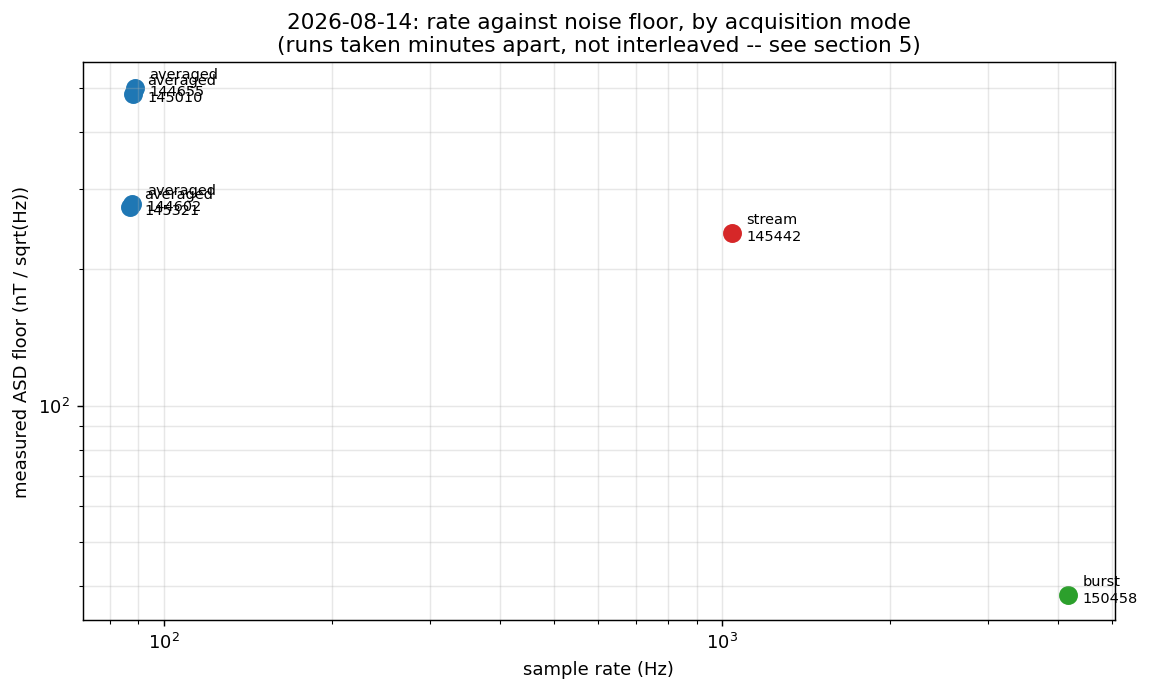
\includegraphics[width=0.86\linewidth]{figures/mode_comparison.png}
\caption{Rate against measured noise floor by method, 2026-08-14. The runs were
taken minutes apart rather than interleaved --- see the warning below.}
\end{figure}

\subsection{The photodiode fix: 4.1\texorpdfstring{$\times$}{x}}

\begin{keybox}[The headline sensitivity result]
Burst-mode noise floor, same two parked points, same measurement:
\[
\text{2026-08-06: } 158\,\text{\etaunit}
\quad\longrightarrow\quad
\text{2026-08-14: } \mathbf{38}\,\text{\etaunit}
\qquad (\mathbf{4.1\times})
\]
attributable to the reference-photodiode gain correction and the removal of signal-diode
saturation. Burst mode is the only method that currently shows the full benefit.
\end{keybox}

\subsection{A warning about comparing these rows}

\begin{openbox}[These runs are not strictly comparable]
They were taken minutes apart, not interleaved, and \S\ref{sec:notshot} shows the
per-rep noise varied \textbf{3.6$\times$} between two averaged runs \textbf{three
minutes apart} with identical settings (145010 vs 145321: 5.97\% vs 2.45\%).

Any A/B comparison across separate runs on this rig is unreliable. Only interleaved
measurements settle a method comparison, which is why the rig test in
\S\ref{sec:rigchecks} interleaves. Treat the method ranking above as indicative.
\end{openbox}

\section{Averaging does not buy \texorpdfstring{$\sqrt{N}$}{sqrt(N)}}

Block-averaging the real burst samples within each burst, 2026-08-06:

\begin{center}
\small
\begin{tabular}{@{}rrrr@{}}
\toprule
\hd{reps averaged} & \hd{$\sigma(\Delta f)$ kHz} & \hd{ideal $1/\sqrt{N}$} & \hd{excess} \\
\midrule
1   & 248.6 & 248.6 & 1.00 \\
4   & 141.0 & 124.3 & 1.13 \\
8   & 110.8 & 87.9  & 1.26 \\
\textbf{23}  & \textbf{86.7} & \textbf{51.8} & \textbf{1.67} \\
64  & 76.5  & 31.1  & 2.46 \\
128 & 72.3  & 22.0  & 3.29 \\
\bottomrule
\end{tabular}
\end{center}

The predicted 86.7\,kHz at $N=23$ matches the averaged runs, which came in at
73--110\,kHz for 11 of 12 runs (median 94\,kHz) --- an independent consistency
check, since the two are measured in completely different modes. But the excess
grows with $N$: past $\sim$30 reps, averaging is nearly free of benefit.

\begin{figure}[H]
\centering
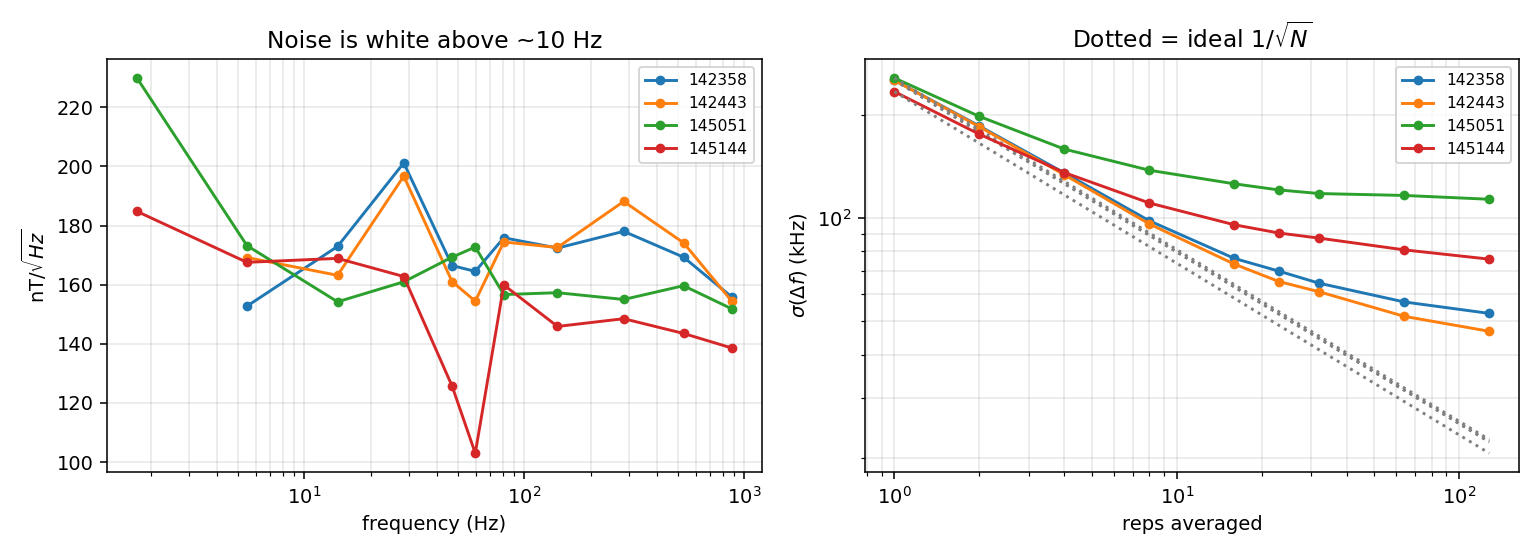
\includegraphics[width=\linewidth]{figures/noise_structure.png}
\caption{Noise spectrum and block-averaging behaviour, 2026-08-06. Above
$\sim$10\,Hz the spectrum is white at $\sim$165\,\etaunit; the excess is all below
10\,Hz.}
\end{figure}

\section{The noise is not photon shot noise}
\label{sec:notshot}

This is the sharpest version of the same finding, and the most important open item
in the document. Per-rep normalised-PL noise, scaled back from whatever averaging
each run used (\file{tables/per_rep_noise.csv}):

\begin{center}
\small
\begin{tabular}{@{}llrrr@{}}
\toprule
\hd{Session} & \hd{Method} & \hd{reps averaged} & \hd{per-rep $\sigma(z)$} & \hd{relative} \\
\midrule
2026-08-06 & burst    & 1  & 0.0076 & \textbf{0.67\%} \\
2026-08-06 & burst    & 1  & 0.0091 & \textbf{0.83\%} \\
2026-08-06 & averaged & 23 & 0.0114 & 1.11\% \\
2026-08-06 & averaged & 23 & 0.0161 & 1.38\% \\
\textbf{2026-08-14} & \textbf{burst} & 1 & \textbf{0.0059} & \textbf{0.61\%} \\
2026-08-14 & averaged & 10 & 0.0214 & 2.45\% \\
2026-08-14 & averaged & 10 & 0.0513 & 5.97\% \\
2026-08-14 & averaged & 23 & 0.0755 & \textbf{8.95\%} \\
2026-08-14 & stream   & 4  & 0.0522 & 7.57\% \\
\bottomrule
\end{tabular}
\end{center}

Two observations:

\begin{enumerate}
  \item \textbf{Burst is reproducibly 0.61--0.83\% in both sessions; everything
        else is 1.1--9\%.} Burst measures the per-rep noise \emph{directly}; the
        other rows infer it by scaling up a reps-averaged $\sigma$. The gap means
        the inference is wrong --- the noise in those modes is not a per-rep term.
  \item \textbf{Averaged mode gets \emph{worse} with more reps} (10 reps
        $\rightarrow$ 2.45\%, 23 reps $\rightarrow$ 8.95\%). Shot noise cannot do
        that.
\end{enumerate}

\begin{openbox}[OPEN --- the per-acquire noise term]
The dominant noise term is \textbf{per-acquire, not per-rep}, so it survives
averaging entirely. \textbf{If it were removed, Method A would inherit Method B's
4$\times$ better noise at no cost in rate}, and free averaging
(\S\ref{sec:freeavg}) would deliver its full $\sqrt{N}$.

Candidate mechanisms, none tested: a start-of-batch transient whose amplitude
varies with the (jittery) idle gap between calls; ADC offset drift re-sampled per
call; laser/MW state settling after the gap. The row-0 transient measured in burst
mode (+1.4\%) is direct evidence that \emph{something} happens at a batch boundary.

Protocol: \S\ref{sec:rigchecks}, check S6.
\end{openbox}

\section{Mains pickup and aliasing}
\label{sec:alias}

From \file{tables/spectra.csv}:

\begin{center}
\small
\begin{tabular}{@{}lrrrl@{}}
\toprule
\hd{Method} & \hd{Rate} & \hd{Strongest line} & \hd{Excess over floor} & \hd{60\,Hz appears at} \\
\midrule
averaged & 86.8--88.8\,Hz & --- & --- & \textbf{26.8--28.8\,Hz (aliased)} \\
stream   & 1041.7\,Hz & 61.7\,Hz & \textbf{10.2$\times$} & 60\,Hz \\
burst    & 4166.7\,Hz & 58.5\,Hz & 3.0$\times$ & 60\,Hz \\
\bottomrule
\end{tabular}
\end{center}

The mains line is real and strong --- \textbf{10$\times$ the noise floor} in the
streamed data, with odd harmonics at 185, 308 and 465\,Hz.

\begin{keybox}[At 88\,Hz, 60\,Hz folds to $\sim$27\,Hz and becomes unfixable]
Nyquist at 87.9\,Hz is 43.9\,Hz, so a 60\,Hz tone aliases to
$|60 - 87.9| = 27.9$\,Hz --- the middle of the measurement band. Once folded there
it is indistinguishable from a real 27.9\,Hz signal, and notching it would remove
real signal along with it.

This is a structural argument for running at $\ge$1\,kHz for drone and MCG work,
\emph{independent of sensitivity}: only there can the pickup be identified for what
it is and removed. \co{twopoint_spectra.alias_report()} raises this automatically
and Step 5A prints it on every averaged run.
\end{keybox}

Note that the 2026-08-06 analysis reported ``no 60\,Hz line''. That was correct for
what it could see: at 87.5\,Hz the line is not \emph{at} 60\,Hz, and the burst runs
of that session, which could have resolved it, were half replays with a badly
compressed time axis. The line was there all along.
